\chapter{Комплексні числа та функції комплексної змінної}
\section{Основні поняття}
$$\underset{\text{натуральні}}{\Nn}\subset\underset{\text{цілі}}{\Zn}\subset\underset{\text{раціональні}}{\Qn}\subset\underset{\text{дійсні}}{\Rn}\subset\underset{\text{комплексні}}{\Cn}$$
$(x,y):x,y\in\Rn$ - пара дійсних чисел.
\begin{figure*}[htp]
	\begin{center}
	\begin{tikzpicture}
		\begin{axis}[ticks=none,axis lines=middle, xmin=-1, xmax=2,ymin=-1,ymax=1.5]
		\end{axis}	
		\draw[-Stealth] (2.29,2.28) -- (5,4) node[midway,above,sloped] {$\rho$};
		\draw (5,4) node[circle,fill,inner sep=0.5pt] {};
		\draw[-Stealth] (2.29,2.28) -- (5,0.56) node[right] {};
		\draw (5,0.56) node[circle,fill,inner sep=0.5pt] {};
		\draw (5,0.56) node[right] {$\bar{z}$};
		\draw (5,4) node[right] {$z$};
		\draw[dashed] (5,4) -- (5,0.56) node[midway, anchor=south west ] {$x$};
		\draw[dashed] (5,4) -- (2.29,4) node[left] {$y$};
		\draw (2.29,2.9) node[circle,fill,inner sep=0.5pt] {};
		\draw (2.29,2.9) node[left] {$i$};
		\draw (3,2.28) arc (0:23:1);
		\draw (3,2.28) node[anchor=south west] {{\tiny$\varphi$}};
		\draw (3,2.28) arc (0:-23:1);
		\draw (3,2.28) node[anchor=north west] {{\tiny$-\varphi$}};
		\draw (2.29,5.4) node[left] {$\Im$};
		\draw (6.5,2.3) node[above] {$\Re$};
		\draw (7,4) node[above] {$z\in\Cn$};
	\end{tikzpicture}
\end{center}
\end{figure*}
$$z=x+iy\textrm{ - алгебраїчна форма }z$$
Якщо $y=0$, то $z=x\in\Rn$. $\Re z=x$ - дійсна частина $z$. Якщо $x=0$, то $z=iy$ - чисто уявне число. $\Im z=y$ - уявна частина $z$. Значення $x,y\in\Rn$ - дійсні. Для $z=i:x=0,y=1,i$ - уявна одиниця. Якщо $z=x+iy$, то $\bar{z}=x-iy$ - спряжене до $z$.
Нехай $\rho,\varphi$ - полярні координати. Тоді модуль $z:|z|=\rho=\sqrt{x^2+y^2}$. $|z|\geq0,\forall z\in\Cn$. Якщо $|z|=0\Leftrightarrow z=0$. $\varphi$ - аргумент $z$ (кут, утворений радіус-вектором, проведеним в точку $z$ у додатньому напрямку з осі $Ox$).\\
$\Arg z$ - множина значень аргумента $z$. $\Arg z=\arg z+2\pi k,k\in\Zn,\arg z$ - головне значення аргумента. $\arg z=\varphi\in(-\pi,\pi]$ 
$$\arg z=\begin{cases}
	\arctan\frac xy,x>0\tab(I,IV\textrm{ чв.})\\\arctan\frac yx+\pi,x<0,y>0\tab(II\textrm{ чв.})\\\arctan\frac yx-\pi,x<0,y<0\tab(III\textrm{ чв.})
\end{cases},\tab\arg z\textrm{ визначений для }z\neq0!$$
$z=\begin{vmatrix}
	x=|z|\cos\varphi\\y=|z|\sin\varphi
\end{vmatrix}=|z|(\cos\varphi+i\sin\varphi)$ - тригонометрична форма числа $z$.

\begin{thm}[Формула Ойлера]
	$$e^{iy}=\cos\varphi+i\sin\varphi\tab(\varphi\in\Rn)$$
\end{thm}
\begin{cons}
	$\\z=|z|e^{i\varphi}$ - показникова форма $z$. $\bar{z}=|z|(\cos(-\varphi+i\sin(-\varphi))=\underset{\textrm{не тригонометрична форма}}{|z|(\cos\varphi-i\sin\varphi)}$. $$\bar{z}=|z|e^{-i\varphi}$$
\end{cons}
\section{Операції над комплексними числами}
\begin{enumerate}
	\item \underline{Порівняння}\\ В комплексній області відношення $">"$ чи $<$ не визначено. Числа порівнюють тільки за допомогою відношення $"="$ або $"\neq"$.
		\begin{align*}
			z_1=z_2\textrm{ у алгебраїчній формі }&\Longleftrightarrow\begin{cases}
				x_1=x_2\\y_1=y_2
			\end{cases}\\
			z_1=z_2\textrm{ у тригонометричній формі }&\Longleftrightarrow\begin{cases}
				|z_1|=|z_2|\\\varphi=\varphi+2\pi k,k\in\Zn
			\end{cases}
		\end{align*}
	\item \underline{Додавання/Віднімання}
		\begin{figure*}[htp]
		\begin{center}
			\begin{tikzpicture}[scale=0.7]
				\begin{axis}[ticks=none,axis lines=middle, xmin=-0.1, xmax=0.5,ymin=-0.1,ymax=1]
				\end{axis}	
				\draw (3.5,6) node[below] {\scriptsize 1: Додавання};
				\draw[-Stealth] (1.15,0.52) -- (4.6,3.65) node[right] {$z_1+z_2$};
				\draw[-Stealth] (1.15,0.52) -- (2.3,2.6) node[left] {$z_2$};
				\draw[dashed] (2.3,2.6) -- (4.6,3.65) node[left] {};
				\draw[-Stealth] (1.15,0.52) -- (3.44,1.55) node[below] {$z_1$};
				\draw[dashed] (3.44,1.55) -- (4.6,3.65) node[left] {};
			\end{tikzpicture}
			\begin{tikzpicture}[scale=0.7]
				\begin{axis}[ticks=none,axis lines=middle, xmin=-0.2, xmax=0.5,ymin=-0.1,ymax=1]
				\end{axis}	
				\draw (4,6) node[below] {\scriptsize 2: Віднімання};
				\draw[-Stealth] (1.95,0.52) -- (3,2.6) node[left] {$z_2$};
				\draw[-Stealth] (1.95,0.52) -- (4.9,1.55) node[right] {$z_1$};
				\draw[-Stealth] (4.9,1.55) -- (3,2.6) node[above,midway,sloped] {$|z_1-z_2|$};
				\draw[-Stealth] (1.95,0.52) -- (0,1.55) node[above,midway,sloped] {$z_2-z_1$};
			\end{tikzpicture}
			\begin{tikzpicture}[scale=0.7]
				\begin{axis}[ticks=none,axis lines=middle, xmin=-0.1, xmax=0.5,ymin=-0.1,ymax=1]
				\end{axis}	
				\draw (3.5,6) node[below] {\scriptsize 3:};
				\draw (5,3) arc (0:360:1.5);
				\draw (3.5,3) node[circle,fill,inner sep=0.5pt] {};
				\draw (3.5,3) node[below] {$z_0$};
				\draw (3.5,3) -- (4.6,4) node[sloped,midway,above] {$R$};
				\draw (4.6,4) node[right] {$z_0$};
			\end{tikzpicture}
		\end{center}
		\end{figure*}
		$$1:z_1+z_2=(x_1+x_2)+i(y_1+y_2)$$
		$$2:z_1-z_2=(x_1-x_2)+i(y_1-y_2)$$
		$$2:|z_1-z_2|=\sqrt{(x_1-x_2)^2+(y_1-y_2)^2}\textrm{ - відстань між }z_1,z_2$$
		$$3:|z-z_0|=R$$
	\item \underline{Множення/ділення і підносення до степеню}\\\\
		$\deff z_1\cdot z_2=\underbrace{x_1x_2-y_1y_2}_{\Re z}+i\underbrace{(x_1y_2+x_2y_1)}_{\Im z}$
		\begin{cons}
			для $z_1=z_2=i:i^2=-1\tab (x_1=x_2=0,y_1=y_2=1)$
		\end{cons}
		\begin{cons}
			$z_1\cdot z_2=x_1x_2+i^2y_1y_2+ix_1y_2+ix_2y_1=x_1(x_2+iy_2)+iy_1(x_2+iy_2)=\\=(x_1+iy_1)(x_2+iy_2)$
		\end{cons}
		Таким чином, комплексні числа перемножаються як звичайні і при цьому \\зберігаються усі формули скороченого множення.\\\\
		$\deff \dfrac{z_1}{z_2}=\dfrac{x_1+iy_1}{x_2+iy_2}\cdot\dfrac{x_2-iy_2}{x_2-iy_2}=\dfrac{A+iB}{x_2^2+y_2^2}=X+iY$\\
		$\deff z^n=(x+iy)^n=\sum\limits_{k=0}^nC_n^kx^k(iy)^{n-k},\tab C_n^k=\dfrac{n!}{k!(n-k)!}\\\left[\begin{array}{l}
			i=i\\i^2=-1\\i^3=-i\\i^4=i\\i^5=1
		\end{array}\right.\dots\left[\begin{array}{l}
			i^{4k}=1\\i^{4k+1}=i\\i^{4k+2}=-1\\i^{4k+3}=-i
		\end{array}\right.$
	\item \underline{Множення/ділення і підносення до степеню (в тригонометричнії і показниковій формі)}\\
		$z_1=|z_1|(\cos\varphi_1+i\sin\varphi_1),z_2=|z_2|(\cos\varphi_2+i\sin\varphi_2).$ Тоді у тригономтричній формі: $z_1\cdot z_2=|z_1|(\cos\varphi_1+i\sin\varphi_1)\cdot |z_2|(\cos\varphi_2+i\sin\varphi_2)=|z_1|\cdot|z_2|\cdot(\cos\varphi_1\cos\varphi_2+\\+i\cos\varphi_1\sin\varphi_2+i\sin\varphi_1\cos\varphi_2+i^2\sin\varphi_1\sin\varphi_2)=|z_1|\cdot|z_2|\cdot((\cos\varphi_1\cos\varphi_2-\sin\varphi_1\sin\varphi_2)++i(\sin\varphi_1\cos\varphi_2+\cos\varphi_1\sin\varphi_2)=|z_1|\cdot|z_2|\cdot(\cos(\varphi_1+\varphi_2)+i\sin(\varphi_1+\varphi_2)\\\\$
		$\deff z_1\cdot z_2=|z_1|\cdot|z_2|\cdot(\cos(\varphi_1+\varphi_2)+i\sin(\varphi_1+\varphi_2))\\\tab\tab\tab\tab\tab\tab|z_1\cdot z_2|=|z_1|\cdot|z_2|,\varphi=\varphi_1+\varphi_2$
		\begin{cons}
			$z_1=z,z_2=\bar{z}\Rightarrow z\cdot\bar{z}=|z|^2(\cos0+i\sin0)=|z|^2$
		\end{cons}
		У показниковій формі(множення):
		$z_1=|z_1|\cdot e^{i\varphi_1},z_2=|z_2|\cdot e^{i\varphi_2}\\\\$
		$\deff z_1\cdot z_2=|z_1|\cdot|z_2|\cdot e^{i(\varphi_!+\varphi_2)}\\$
		У тригонометричній формі(ділення): $\dfrac{z_1}{z_2}=\dfrac{|z_1|}{|z_2|}\cdot\dfrac{\cos\varphi_1+i\sin\varphi_1}{\cos\varphi_2-i\sin\varphi_2}=\dfrac{|z_1|}{|z_2|}\cdot\\\dfrac{(\cos\varphi_1+i\sin\varphi_1)(\cos\varphi_2+i\sin\varphi_2)}{\cos^2\varphi_2+\sin^2\varphi_2}=\dfrac{|z_1|}{|z_2|}\cdot(\cos\varphi_1+i\sin\varphi_1)\cdot(\cos(-\varphi_2)+i\sin(-\varphi_2))\\\\$
		$\deff \dfrac{z_1}{z_2}=\dfrac{|z_1|}{|z_2|}(\cos(\varphi_1-\varphi_2)+i\sin(\varphi_1-\varphi_2))),\tab\left|\dfrac{z_1}{z_2}\right|=\dfrac{|z_1|}{|z_2|},\varphi=\varphi_1-\varphi_2\\\\$
		У показниковій формі(ділення):\\\\
		$\deff \dfrac{z_1}{z_2}=\dfrac{|z_1|}{|z_2|}\cdot e^{i(\varphi_1-\varphi_2)}\\\\$
		$\deff z^n=\underbrace{z\cdot z\cdot z\cdot\dots\cdot z }_{n\textrm{ разів}}=|z|^n(\cos n\varphi+i\sin n\varphi)=|z|^n\cdot e^{in\varphi},\forall n\in\Zn$
	\item \underline{Винесення з під кореня $\sqrt[n]{z}$}\\\\
		$\deff W=\sqrt[n]{z},$ якщо $W^n=z$.\\\\
		Нехай обидва записані у тригонометричній формі: $z=|z|(\cos\varphi+i\sin\varphi),\\W=|W|(\cos\psi+i\sin\psi),W^n=|W|^n(\cos n\psi+i\sin n\psi)$. Умова "=" в тригоно-\\-метричній формі: $W^n=z\Rightarrow\left\{\begin{array}{l}
			|W|^n=|z|\\n\psi=\varphi+2\pi k,k\in\Zn
		\end{array}\right.\Rightarrow\left\{\begin{array}{l}
			|W|=\sqrt[n]{|z|}\\\psi=\dfrac{\varphi+2\pi k}{n},k\in\Zn
		\end{array}\right.$
	\begin{figure*}[htp!]
		\begin{wrapfigure}[11]{l}{0.4\textwidth} 
    		\centering
    		\begin{tikzpicture}[scale=0.8]
    			\begin{axis}[ticks=none,axis lines=middle, xmin=-0.5, xmax=0.5,ymin=-0.5,ymax=0.5]
				\end{axis}	
				\draw (4.5,3.6) node[below] {\tiny$\dfrac{2\pi}{n}$};
				\draw (4,4.1) node[below] {\tiny$\dfrac{2\pi}{n}$};
				\draw (4.9,2.9) arc (0:360:1.5);
				\draw (3.9,2.85) arc (0:108:0.5);
				\draw (3.43,2.85) node[circle,fill,inner sep=0.5pt] {};
				\draw (4.64, 3.74) node[circle,fill,inner sep=0.5pt] {};
				\draw (3.88, 4.32) node[circle,fill,inner sep=0.5pt] {};
				\draw (2.88, 4.31) node[circle,fill,inner sep=0.5pt] {};
				\draw (3.43,2.85) -- (4.65, 3.75) node[above, right] {\scriptsize$\dfrac{\varphi}{n}(k=0)$};
				\draw (3.43,2.85) -- (3.88, 4.33) node[above] {\scriptsize$k=1$};
				\draw (3.43,2.85) -- (2.88, 4.31) node[above] {\scriptsize$k=2$};
    		\end{tikzpicture}
		\end{wrapfigure}$\\\\\sqrt[n]{z}=W=\sqrt[n]{|z|}\left(\cos\dfrac{\varphi+2\pi k}{n}+i\sin\dfrac{\varphi+2\pi k}{n}\right)\\k=0,1,\dots,n-1\\\psi_k=\dfrac{\varphi}{n}+2\pi\dfrac{k}{n},\tab\Delta\psi=\dfrac{2\pi}{n}\\$
	\end{figure*}
	\begin{example}
		\begin{wrapfigure}{l}{0.5\textwidth} 
			\centering
    		\begin{tikzpicture}[scale=0.4]
    			\begin{axis}[ticks=none,axis lines=middle,thick, xmin=-1, xmax=1,ymin=-1,ymax=1]
				\end{axis}	
				\draw (3.43,2.85) node[circle,fill,inner sep=0.5pt] {};
				\draw (3.43,1.4) node[circle,fill,inner sep=0.5pt] {};
				\draw (3.43,4.4) node[circle,fill,inner sep=0.5pt] {};
				\draw (1.9,2.85) node[circle,fill,inner sep=0.5pt] {};
				\draw (4.9,2.85) node[below] {\scriptsize1};
				\draw (4.9,2.85) node[circle,fill,inner sep=0.5pt] {};
    		\end{tikzpicture}
		\end{wrapfigure}
		$\\\\\\\sqrt[4]{1}=\Delta\varphi=\dfrac{2\pi}{4}=\dfrac{\pi}{2}\\$
	\end{example}
\end{enumerate}
\section{Послідовності комплексних чисел}
Послідовність комплексних чисел --- це комплекснозначна функція натурального аргумента. $\{z_n\}$ - послідовність.\\\\
$\deff n\in\Nn\rightarrow f(n)=z_n\in\Cn$
\begin{enumerate}
	\item \tab\begin{figure*}[htp!]
		\begin{wrapfigure}{l}{0.4\textwidth} 
			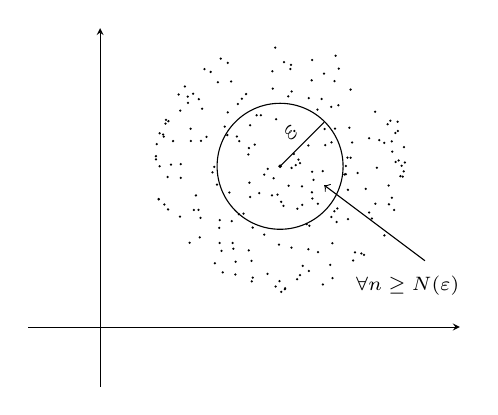
\begin{tikzpicture}[scale=0.8]
				\begin{axis}[ticks=none,axis lines=middle, xmin=-0.1, xmax=0.5,ymin=-0.1,ymax=0.5,xshift=-4cm]
				\end{axis}	
				\draw (1,3.5) arc (0:360:1);
				\draw (0,3.5) node[circle,fill,inner sep=0.5pt] {};
				\draw (0,3.5) -- (0.7,4.2) node[midway,sloped,above] {$\varepsilon$};
				\draw[->] (2.3, 2) -- (0.7,3.2);
				\draw (3, 1.6) node[below,left] {\scriptsize$\forall n\geq N(\varepsilon)$};
				\pgfmathsetseed{24122015}
    			\foreach \p in {1,...,200}
    			{ \pgfmathsetmacro{\x}{2*rand}
        			\pgfmathsetmacro{\y}{-rand*sqrt(4-pow(\x,2))+3.5}
        			\fill[black]    (\x,\y) circle (0.02);
    			}
			\end{tikzpicture}
		\end{wrapfigure}
		$\\\\\limntoinf z_n=z_0,z_0\in\Cn\\\\\tab\tab\Updownarrow\\\\\forall\varepsilon\tab\exists N=N(\varepsilon)\in\Nn:\forall n\geq N(\varepsilon)\tab|z_n-z_0|<\varepsilon$
	\end{figure*}\newpage
	\item \tab\begin{figure*}[htp]
		\begin{wrapfigure}{l}{0.4\textwidth} 
			\begin{tikzpicture}[scale=0.8]
			\begin{axis}[ticks=none,axis lines=middle, xmin=-0.5, xmax=0.5,ymin=-0.5,ymax=0.5,xshift=-3.4cm]
			\end{axis}
			\pgfmathsetseed{24122015}
    		\foreach \p in {1,...,200}
   			{ \pgfmathsetmacro{\x}{2*rand}
       			\pgfmathsetmacro{\y}{-rand*sqrt(4-pow(\x,2))+2.8}
       			\fill[black]    (\x,\y) circle (0.02);
   			}
   			\draw (0,2.8) circle (1);
   			\draw (0.9,3.1) node[right] {\scriptsize$M$};
   			\draw (1,2.85) node[circle,fill,inner sep=1pt] {};
		\end{tikzpicture}
		\end{wrapfigure}
		$\\\\\\{z_n}$ - обмежена, якщо $\\\\\exists M>0\tab\forall n\in\Nn\tab|z_n|<M$
	\end{figure*}\\
\end{enumerate}$\\$
\begin{thm}\label{thm:zn+z0}
	\begin{align*}
		\textrm{Нехай}\tab& z_n=x_n+iy_n,&\\
		&z_0=x_0+iy_0,&(x_n,y_n,x_0,y_0\in\Rn)\\
		\textrm{Тоді:}\tab& \limntoinf z_n=z_0\tab\Longleftrightarrow\tab 
		\begin{cases}
			\limntoinf x_n=x_0\\\limntoinf y_n=y_0
		\end{cases}
	\end{align*}
\end{thm}
\begin{figure*}[htp]
	\begin{center}
		\begin{tikzpicture}[scale=1]
				\begin{axis}[ticks=none,axis lines=middle, xmin=-0.1, xmax=0.5,ymin=-0.1,ymax=1]
				\end{axis}	
				\draw (4,5) node[below] {$|z_1+z_2|\leq|z_1|+|z_2|$};
				\draw[-Stealth] (1.15,0.52) -- (4.6,3.65) node[above,midway,sloped] {\tiny$|z_1+z_2|$} node[right] {$z_1+z_2$};
				\draw[-Stealth] (1.15,0.52) -- (2.3,2.6) node[above,midway,sloped] {\tiny$|z_2|$} node[left] {$z_2$};
				\draw[dashed] (2.3,2.6) -- (4.6,3.65) node[left] {};
				\draw[-Stealth] (1.15,0.52) -- (3.44,1.55) node[above,midway,sloped] {\tiny$|z_1|$} node[below] {$z_1$};
				\draw[dashed] (3.44,1.55) -- (4.6,3.65) node[left] {};
			\end{tikzpicture}
			\caption*{До доведення \cref{thm:zn+z0}}
	\end{center}
\end{figure*}
\begin{prooff}$ $
	\begin{enumerate}[label=\alph*)]
		\item необхідність:\\
			Нехай $\limntoinf z_n=z_0$, тобто $\forall\varepsilon>0\tab\exists N(\varepsilon)\in\Nn\tab\forall n\geq N(\varepsilon)\tab|z_n-z_0|<\varepsilon\\|z_n-z_0|=|(x_n+iy_n)-(x_0+iy_0)|=|(x_n-x_0)+i(y_n-y_0)|\Longrightarrow\\\Longrightarrow\sqrt{(x_n-x_0)^2+i(y_n-y_0)^2}<\varepsilon ,\tab (x_n-x_0)^2+i(y_n-y_0)^2<\varepsilon^2\Longrightarrow\\\Longrightarrow\begin{cases}
				(x_n-x_0)^2<\varepsilon^2\\(y_n-y_0)^2<\varepsilon^2
			\end{cases}\Longrightarrow\begin{cases}
				|x_n-x_0|<\varepsilon\\|y_n-y_0|<\varepsilon
			\end{cases},\forall n\geq N(\varepsilon)\tab\Longleftrightarrow$
			\begin{center}
				$\Longleftrightarrow\tab \begin{cases}
			\limntoinf x_n=x_0\\\limntoinf y_n=y_0
			\end{cases}$
			\end{center}
		\item достатність:\\Нехай $\begin{cases}
			\limntoinf x_n=x_0\\\limntoinf y_n=y_0
			\end{cases}\tab\begin{array}{ll}
				\forall\varepsilon>0:&\exists N_1(\varepsilon)\in\Nn:\forall n\geq N_1(\varepsilon)\tab |x_n-x_0|<\frac{\varepsilon}{2} \\
				&\exists N_2(\varepsilon)\in\Nn:\forall n\geq N_2(\varepsilon)\tab |y_n-y_0|<\frac{\varepsilon}{2}
			\end{array}\\|z_n-z_0|=|(x_n+iy_n)-(x_0+iy_0)|=|(x_n-x_0)+i(y_n-y_0)|\leq\\\leq|x_n-x_0|+|i|\cdot|y_n-y_0|=|x_n-x_0|+|y_n-y_0|<\dfrac{\varepsilon}{2}+\dfrac{\varepsilon}{2}=\varepsilon$. \\при $\forall n\geq\max(N_1,N_2)\Longrightarrow\limntoinf z_n=z_0$
	\end{enumerate}
\end{prooff}
\begin{statement}
	$$\limntoinf z_n=z_0\Longleftrightarrow\limntoinf|z_n-z_0|=0$$
\end{statement}
\begin{prooff}
	$\\\forall\varepsilon>0\tab\exists N(\varepsilon)\in\Nn:\forall n\geq N(\varepsilon)\tab|z_n-z_0|<\varepsilon$. Тоді: $||z_n-z_0|-0|=|z_n-z_0|<\varepsilon$
\end{prooff}
\begin{thm}\label{thm:zn-z0}
	$$\textrm{Якщо }\limntoinf z_n=z_0,\textrm{ то }\limntoinf|z_n|=|z_0|$$
\end{thm}
\begin{figure*}[htp]
	\begin{center}
		\begin{tikzpicture}
				\begin{axis}[ticks=none,axis lines=middle, xmin=-0.2, xmax=0.5,ymin=-0.1,ymax=1]
				\end{axis}	
				\draw[-Stealth] (1.95,0.52) -- (3,2.6) node[above,midway,sloped] {\tiny$|z_n|$} node[left] {$z_n$};
				\draw[-Stealth] (1.95,0.52) -- (4.9,1.55) node[below,midway,sloped] {\tiny$|z_0|$} node[right] {$z_0$};
				\draw[-Stealth]  (4.9,1.55) -- (3,2.6) node[above,midway,sloped] {$|z_n-z_0|$};
			\end{tikzpicture}
			\caption*{До доведення \cref{thm:zn-z0}}
	\end{center}
\end{figure*}
\begin{prooff}$\\$
	Покажемо, що $\limntoinf||z_n|-|z_0||=0$ (у зворотний бік невірно).\\
	$\left.\begin{array}{ll}
		\textrm{Нерівність }\triangle \textrm{ для }|z_n|:&|z_n|\leq|z_0|+|z_n-z_0|\\&|z_n|-|z_0|\leq|z_n-z_0|\\\textrm{Нерівність }\triangle \textrm{ для }|z_-0|:&|z_0|\leq|z_n|+|z_n-z_0|\\&|z_0|-|z_n|\leq|z_n-z_0|
	\end{array}\right\}\Longrightarrow||z_n|-|z_0||\leq|z_n-z_0|$\\
	Окрім того, $0\leq||z_n|-|z_0||\leq|z_n-z_0|\Longrightarrow(\limntoinf0=0,\limntoinf|z_n-z_0|=0$ - за умовою) $\Longrightarrow\limntoinf||z_n|-|z_0||=0\Longleftrightarrow\limntoinf|z_n|=|z_0|$
\end{prooff}
\begin{thm}
	$$\begin{cases}
		\limntoinf|z_n|=|z_0|\\\limntoinf\varphi_n=\varphi_0
	\end{cases}\xRightarrow[\begin{array}{l}
		{\scriptscriptstyle z_n=|z_n|\cdot e^{i\varphi_n}}\\{\scriptscriptstyle z_0=|z_0|\cdot e^{i\varphi_0}}
	\end{array}]{}\limntoinf z_n=z_0$$
\end{thm}
\begin{prooff}
	З арифметичних властивостей $\lim z_n$
\end{prooff}
\section{Розширена множина $\Cn$. Нескінченно віддалена точка.}
\begin{figure*}[htp!]
		\begin{wrapfigure}{l}{0.45\textwidth} 
			\begin{tikzpicture}
				\begin{axis}[ticks=none,axis lines=middle, xmin=-1, xmax=1,ymin=-1,ymax=1,xshift=-3.4cm]
				\end{axis}	
				\draw (0,2.9) circle (30pt);
				\draw[->] (3, 5) -- (2,4);
				\draw (3, 5) node[right,above] {\scriptsize$\forall n\geq N(\varepsilon)$};
				\pgfmathsetseed{24122015}
    			\foreach \p in {1,...,200}
    			{ \pgfmathsetmacro{\x}{2*rand}
        			\pgfmathsetmacro{\y}{-rand*sqrt(4-pow(\x,2))+2.9}
        			\fill[black]    (\x,\y) circle (0.02);
    			}
			\end{tikzpicture}
		\end{wrapfigure}
		$\\\\\limntoinf z_n=\infty\Leftrightarrow\forall E>0\tab\exists N(E)\in\Nn\\\forall n\geq N(E)\tab |z_n|>\varepsilon.$ Невласне комплексне число $\infty$: поняття дійсної та уявної частини, а також, аргумента - невизначені. $|\infty|=\infty.\tab \limntoinf z_n=\infty\Rightarrow\limntoinf|z_n|=+\infty.\tab\limntoinf\dfrac1{z_n}=0\\\\\\$
\end{figure*}
\begin{figure*}[htp]
	\begin{wrapfigure}{l}{0.65\textwidth} 
		\underline{Операції} над $"\infty"$ і $a\in\Cn:\\\\$
	$\deff "\infty\pm a"=\infty\\\deff"\infty\cdot a=\infty,\tab a\neq0"\\\deff"\dfrac\infty a"=\infty\\\deff"\dfrac a\infty"=0\\\deff"\infty\cdot\infty"=\infty\\\\$
	\end{wrapfigure}
	$\\$\underline{Невизначеності}: $0\cdot\infty,\tab\dfrac\infty\infty,\tab\dfrac00,\tab \infty+\infty,\tab\infty-\infty.\\\\\\\\$
\end{figure*}

\begin{figure*}[htp]\centering
	\begin{tikzpicture}
		\begin{axis}[ticks=none,axis lines=middle, xmin=-0.1, xmax=0.9,ymin=-0.5,ymax=0.5]
				\end{axis}
				\draw (3.5,0) -- (3.5,5.5);
				\draw[->] (0.69,2.85) -- (3.5,5);
				\draw[->] (0.69,2.85) -- (3.5,4.5);
				\draw[->] (0.69,2.85) -- (3.5,4);
				\draw[->] (0.69,2.85) -- (3.5,0.7);
				\draw[->] (0.69,2.85) -- (3.5,1.2);
				\draw[->] (0.69,2.85) -- (3.5,1.7);
				\draw (4.5,2.85) node[circle,fill,inner sep=1pt] {};
				\draw (5,2.85) node[circle,fill,inner sep=1pt] {};
				\draw (5.5,2.85) node[circle,fill,inner sep=1pt] {};
				\draw (5,4) node {\scriptsize результат};
				\draw (5,3.5) node {\scriptsize (постійна)};
	\end{tikzpicture}\tab
	\begin{tikzpicture}
		\coordinate (P) at ({1/sqrt(3)},{1/sqrt(3)},{1/sqrt(3)});
 
% Draw circle
		\draw (0,1,0) circle (1cm);
% draw arcs 		
		\tdplotsetrotatedcoords{0}{0}{0};
		\draw[dashed, tdplot_rotated_coords, gray] (0,0,1) circle (1);
% Axes in 3 d coordinate system
		\draw[-stealth] (0,0,0) -- (4,0,0) node[below left] {$x$}; 
		\draw[-stealth] (0,0,0) -- (0,3,0) node[below right] {$y$};
		\draw[-stealth] (0,0,0) -- (0,0,5) node[above] {$z$};
% nodes		
		\draw (0,1,0) node[circle,fill,inner sep=1pt] {};
		\draw (0,2,0) node[circle,fill,inner sep=1pt] {};
		\draw (1.2,0.97,1) node[circle,fill,inner sep=1pt] {};
		\draw (3,0,3) node[circle,fill,inner sep=1pt] {};
		\draw (3,3,0) node {$z\leftrightarrow z'$};
		\draw (3,2,0) node {$\infty\leftrightarrow N$};
		\draw (3,-2,0) node {\scriptsize$N$ образ нескінченно відадаленої точки};
% lines		
		\draw[dashed]  (0,2,0) node[anchor=south west] {$N$} -- (1.2,0.97,1);
		\draw (1.2,0.97,1) -- (3,0,3) node[below] {$z$};
		\draw[->] (1.2,0.97,1) -- (2,0.5,-0.5) node[right] {$z'$};

	\end{tikzpicture}
\end{figure*}\newpage
\section{}






























